% Appendix 1: 2D parametric curves (enrichment; outside NESA syllabus)
\begingroup
\scriptsize
\setlength{\parskip}{0pt}
\setlength{\parindent}{0pt}

\noindent\fbox{%
\begin{minipage}{0.97\textwidth}
\textit{\textbf{Enrichment only.} These 2D parametric curves are \textbf{outside the current NESA Mathematics Extension~1 and Extension~2 syllabuses}. They are included for students interested in university mathematics, physics, engineering, and computer graphics.}
\end{minipage}}

\vspace{0.25em}

% Row 1
\noindent
\begin{minipage}[t]{0.48\textwidth}
\centering
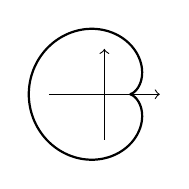
\begin{tikzpicture}[scale=0.32,baseline=(current bounding box.center)]
  \draw[thin,->] (-2.2,0) -- (2.2,0);
  \draw[thin,->] (0,-1.8) -- (0,1.8);
  \draw[thick,domain=0:360,samples=120,smooth]
    plot ({2*cos(\x)-cos(2*\x)},{2*sin(\x)-sin(2*\x)});
\end{tikzpicture}\\[-0.1em]
\textbf{Cardioid}\\[-0.1em]
\scriptsize Heart-shaped curve from a rolling circle.\\[0.1em]
$x=a(2\cos t-\cos 2t)$\\
$y=a(2\sin t-\sin 2t)$
\end{minipage}\hfill
\begin{minipage}[t]{0.48\textwidth}
\centering
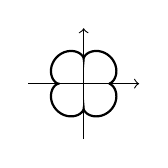
\begin{tikzpicture}[scale=0.32,baseline=(current bounding box.center)]
  \draw[thin,->] (-2.2,0) -- (2.2,0);
  \draw[thin,->] (0,-2.2) -- (0,2.2);
  \draw[thick,domain=0:360,samples=120,smooth]
    plot ({1.25*cos(\x)-0.25*cos(5*\x)},{1.25*sin(\x)-0.25*sin(5*\x)});
\end{tikzpicture}\\[-0.1em]
\textbf{Epicycloid}\\[-0.1em]
\scriptsize Curve traced by a point on a circle rolling outside another.\\[0.1em]
$x=(a+b)\cos t-b\cos\!\bigl(\tfrac{a}{b}+1\bigr)t$\\
$y=(a+b)\sin t-b\sin\!\bigl(\tfrac{a}{b}+1\bigr)t$
\end{minipage}

\vspace{0.15em}

% Row 2
\noindent
\begin{minipage}[t]{0.48\textwidth}
\centering
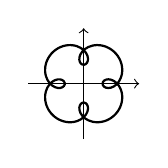
\begin{tikzpicture}[scale=0.32,baseline=(current bounding box.center)]
  \draw[thin,->] (-2.2,0) -- (2.2,0);
  \draw[thin,->] (0,-2.2) -- (0,2.2);
  \draw[thick,domain=0:360,samples=120,smooth]
    plot ({1.25*cos(\x)-0.5*cos(5*\x)},{1.25*sin(\x)-0.5*sin(5*\x)});
\end{tikzpicture}\\[-0.1em]
\textbf{Epitrochoid}\\[-0.1em]
\scriptsize Epicycloid with the tracing point offset from the rolling circle.\\[0.1em]
$x=(a+b)\cos t-c\cos\!\bigl(\tfrac{a}{b}+1\bigr)t$\\
$y=(a+b)\sin t-c\sin\!\bigl(\tfrac{a}{b}+1\bigr)t$
\end{minipage}\hfill
\begin{minipage}[t]{0.48\textwidth}
\centering
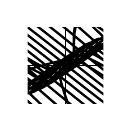
\begin{tikzpicture}[scale=0.32,baseline=(current bounding box.center)]
  \clip (-1.5,-1.5) rectangle (1.5,1.5);
  \draw[thin,->] (-1.8,0) -- (1.8,0);
  \draw[thin,->] (0,-1.8) -- (0,1.8);
  \draw[thick,domain=-20:160,samples=120,smooth]
    plot ({3*cos(\x r)/(1+sin(\x r)^3)},{3*sin(\x r)*cos(\x r)/(1+sin(\x r)^3)});
\end{tikzpicture}\\[-0.1em]
\textbf{Folium of Descartes}\\[-0.1em]
\scriptsize A loop with an oblique asymptote.\\[0.1em]
Cartesian: $x^3+y^3=3axy$\\[0.1em]
$x(t)=\dfrac{3at}{1+t^3}$, \quad $y(t)=\dfrac{3at^2}{1+t^3}$
\end{minipage}

\vspace{0.15em}

% Row 3
\noindent
\begin{minipage}[t]{0.48\textwidth}
\centering
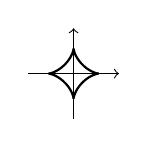
\begin{tikzpicture}[scale=0.32,baseline=(current bounding box.center)]
  \draw[thin,->] (-1.8,0) -- (1.8,0);
  \draw[thin,->] (0,-1.8) -- (0,1.8);
  \draw[thick,domain=0:360,samples=120,smooth]
    plot ({0.75*cos(\x)+0.25*cos(3*\x)},{0.75*sin(\x)-0.25*sin(3*\x)});
\end{tikzpicture}\\[-0.1em]
\textbf{Hypocycloid}\\[-0.1em]
\scriptsize Curve from a circle rolling inside a fixed circle.\\[0.1em]
$x=(a-b)\cos t+b\cos\!\bigl(\tfrac{a}{b}-1\bigr)t$\\
$y=(a-b)\sin t-b\sin\!\bigl(\tfrac{a}{b}-1\bigr)t$
\end{minipage}\hfill
\begin{minipage}[t]{0.48\textwidth}
\centering
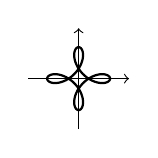
\begin{tikzpicture}[scale=0.32,baseline=(current bounding box.center)]
  \draw[thin,->] (-2.0,0) -- (2.0,0);
  \draw[thin,->] (0,-2.0) -- (0,2.0);
  \draw[thick,domain=0:360,samples=120,smooth]
    plot ({0.75*cos(\x)+0.5*cos(3*\x)},{0.75*sin(\x)-0.5*sin(3*\x)});
\end{tikzpicture}\\[-0.1em]
\textbf{Hypotrochoid}\\[-0.1em]
\scriptsize Hypocycloid with the tracing point offset from the rolling circle.\\[0.1em]
$x=(a-b)\cos t+c\cos\!\bigl(\tfrac{a}{b}-1\bigr)t$\\
$y=(a-b)\sin t-c\sin\!\bigl(\tfrac{a}{b}-1\bigr)t$
\end{minipage}

\vspace{0.15em}

% Row 4
\noindent
\begin{minipage}[t]{0.48\textwidth}
\centering
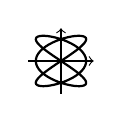
\begin{tikzpicture}[scale=0.32,baseline=(current bounding box.center)]
  \draw[thin,->] (-1.3,0) -- (1.3,0);
  \draw[thin,->] (0,-1.3) -- (0,1.3);
  \draw[thick,domain=0:360,samples=120,smooth]
    plot ({sin(3*\x)},{sin(2*\x)});
\end{tikzpicture}\\[-0.1em]
\textbf{Lissajous Curves}\\[-0.1em]
\scriptsize Closed curves from harmonic motion in two perpendicular directions.\\[0.1em]
$x(t)=a\sin(nt+c)$, \quad $y(t)=b\sin t$
\end{minipage}\hfill
\begin{minipage}[t]{0.48\textwidth}
\centering
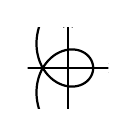
\begin{tikzpicture}[scale=0.32,baseline=(current bounding box.center)]
  \clip (-1.6,-1.6) rectangle (1.6,1.6);
  \draw[thin,->] (-1.8,0) -- (1.8,0);
  \draw[thin,->] (0,-1.8) -- (0,1.8);
  \draw[thick,domain=25:155,samples=100,smooth]
    plot ({sin(5*\x)/sin(\x)},{2*sin(3*\x)*sin(2*\x)/sin(\x)});
\end{tikzpicture}\\[-0.1em]
\textbf{Plateau Curves}\\[-0.1em]
\scriptsize Rose-like curves from rational trigonometric combinations.\\[0.1em]
$x(t)=\dfrac{a\sin((m+n)t)}{\sin((m-n)t)}$\\[0.1em]
$y(t)=\dfrac{2a\sin(mt)\sin(nt)}{\sin((m-n)t)}$
\end{minipage}

\endgroup
